\chapter{Experiments and results}
	% \gjor{Vurder å dele opp som Tønnes: Først 1) Evolusjonære/\opphoy{Simulator} eksperimenter og resultater, så 2) Fysiske eksperiment og resultater}
	
	\section{Solving the simpler $\phi-$problem}
	This is the section for the experiments attempting to solve the first and simpler problem, namely synchronizing the phases $\phi_i$ of all agents $i$. \nl
	
	\begin{figure}[ht!]
		\centering
		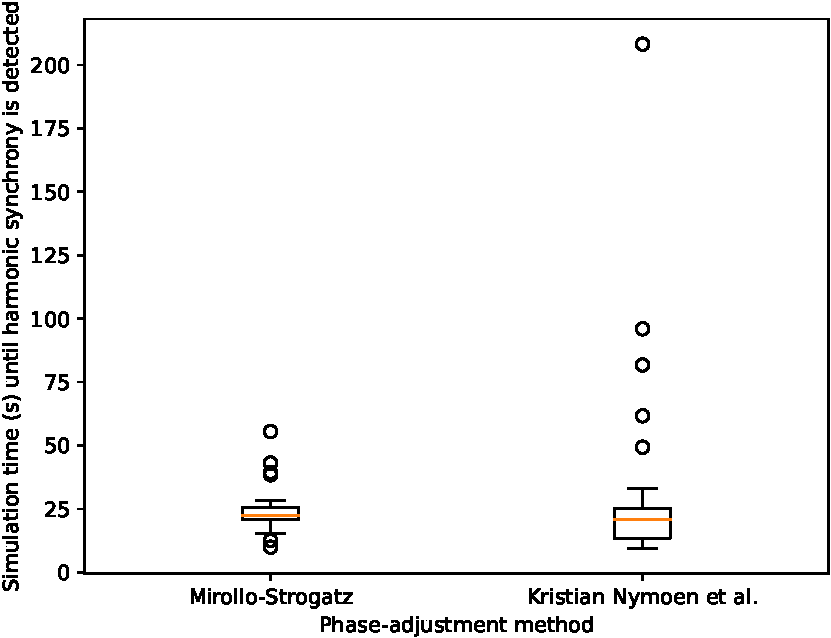
\includegraphics[width=0.7\linewidth]{Assets/Figures/Experiments/FirstExperimentPlot.pdf}
		\caption{Performance-plot: harmonic synchronization-times from initial simulator-experiment when synchronizing phases $\phi_i$ for all agents $i$, where all phases are initially uniformly randomized between 0 and 1, and eventually synchronize and align. We here measure how long it takes 6 agents to synchronize their phases to each other, given the two different phase-adjustment methods. 30 individual runs per phase-adjustment method were performed in Unity for a collective-size of 6 agents, and $\alpha=0.2$ e.g.}
		\label{fig:EPA1}
	\end{figure}
	
	
	\section{Solving the harder $\phi\&\omega-$problem}
	
	This is the section for the experiments attempting to solve the second and harder problem of synchronizing both phases $\phi_i$, as well as frequencies $\omega_i$, for all agents $i$.